%% !TEX program = lualatex
\documentclass[
    %answers,
    a4paper,ngerman,11pt, addpoints]{exam}

\usepackage[utf8]{inputenc}
%\usepackage[T1]{fontenc}
%\usepackage[ngerman]{babel}


\usepackage{polyglossia}
\setdefaultlanguage[variant = swiss]{german}
\usepackage{fontspec}
\setmainfont{Arial} % Bauschule CI Manual
\setsansfont{Arial} % Bauschule CI Manual


\usepackage[ a4paper,
 total={165mm,250mm},
 left=25mm,
 top=25mm,
 headsep=10mm
 %footsep=12mm
 %,showframe
  ]{geometry}

\usepackage{graphicx}
\usepackage{siunitx}
\usepackage{booktabs} % schöne Tabellen
\usepackage{float}
\floatplacement{figure}{H}
\usepackage{xcolor}
\usepackage{pdfpages}
\usepackage{enumitem}
\usepackage{mdframed} % Boxen
\usepackage{amsmath,amssymb}
\usepackage{tcolorbox}
\usepackage{lastpage} % For the total number of pages
\usepackage{gensymb}
\usepackage{xspace}
\usepackage{tabularx}
\usepackage{multicol}
\usepackage[
    version=3,
    arrows=pgf-filled,
]{mhchem} % für chemische Formeln
%\usepackage{microtype}
\usepackage{subfigure}
\usepackage[hidelinks]{hyperref}
\usepackage{cleveref}
\usepackage{luacode}
\usepackage{amsmath}
\usepackage{textcomp}


\sisetup{
  locale = DE,
  inter-unit-product = \ensuremath{{\cdot}},
  detect-all,
}

% Colors
\definecolor{blau_bauschule}{RGB}{22,65,148}
\CorrectChoiceEmphasis{\color{blau_bauschule}}
\SolutionEmphasis{\color{blau_bauschule}}

\setlength{\parindent}{0em} % Verhindert einrücken
\setlength\linefillheight{0.3in}


%% COMMMANDS
\author{Patrick Pfändler}
\newcommand{\dozent}{Patrick Pfändler}
\newcommand{\fach}{Baustoffe}


\newcommand{\punkte}[1]{%
    \begin{infobox}%
        #1
    \end{infobox}}%
\newcommand{\FinRes}[1]{\underline{\underline{#1}}}

\newmdenv[linecolor=black,backgroundcolor=gray!15,frametitle={Punktverteilung},leftmargin=1cm,rightmargin=1cm]{infobox}

\newcommand{\pagebreaksol}{
    \ifprintanswers
        \clearpage
    \else
        {}
    \fi
}

\newcommand{\pagebreakexam}{
    \ifprintanswers
        {}
    \else
        \clearpage
    \fi
}

\SolutionEmphasis{\color{blau_bauschule}}
\makeatletter%
\newcommand{\solutiontable}[1]{\ifprintanswers\begingroup\Solution@Emphasis#1\if@shadedsolutions%
            {\cellcolor{SolutionColor}}%
        \else%
        \fi\endgroup\else\phantom{#1}\fi}%
\makeatother%

\newcommand{\myNmm}[1]
{
    \sisetup{per-mode=symbol}
    \SI{#1}{\newton\per\mm\squared}
}

\renewcommand{\thequestion}{\fontsize{12pt}{2pt} \selectfont  \bfseries \arabic{question}}
\sisetup{per-mode=symbol}



%% Translation

\pointpoints{Punkt}{Punkte}
\bonuspointpoints{Bonuspunkt}{Bonuspunkte}
\renewcommand{\solutiontitle}{\noindent\textbf{Lösung:}\enspace}
\chqword{Frage}
\chpgword{Seite}
\chpword{Punkte}
\chbpword{Bonus Punkte}
\chsword{Erreicht}
\chtword{Gesamt}
\hpword{Punkte:}
\hsword{Ergebnis:}
\hqword{Aufgabe:}
\htword{Summe:}


\renewcommand{\questionshook}{%
  %\setlength{\leftmargin}{0pt}% removes the indentation from the left
  \setlength{\labelwidth}{1.25cm}% adjusts label width
  \setlength{\itemindent}{0cm}% aligns the start of the item with the above
  \setlength{\labelsep}{0.25cm}% space between the label and the item text
}




%% header and footer
\pagestyle{headandfoot}
\firstpageheadrule
\runningheadrule

% Adjust the font size for the header
\firstpageheader{\fontsize{9}{11}\selectfont\fach}{}{\fontsize{9}{11}\selectfont\dozent \\ \blattname}
\runningheader{\fontsize{9}{11}\selectfont\fach}{}{\fontsize{9}{11}\selectfont\dozent \\ \blattname}

% Adjust the font size for the footer
\firstpagefooter{
\includegraphics[width=2.5cm]{bauschule-logo-5cm.png}}{}{\fontsize{9}{11}\selectfont\thepage\,/\,\pageref{LastPage}}
\runningfooter{
\includegraphics[width=2.5cm]{bauschule-logo-5cm.png}}{}{\fontsize{9}{11}\selectfont\thepage\,/\,\pageref{LastPage}}
% !TEX root = /Users/patricpf/Documents/repos/Bauschule-Baustoffe/Unterlagen/09_Metalle/Aufgaben/Stahlzug/Zugversuch.tex
% !TEX program = lualatex
\documentclass[
    %answers,
    a4paper,ngerman,11pt, addpoints]{exam}

\usepackage[utf8]{inputenc}
%\usepackage[T1]{fontenc}
%\usepackage[ngerman]{babel}


\usepackage{polyglossia}
\setdefaultlanguage[variant = swiss]{german}
\usepackage{fontspec}
\setmainfont{Arial} % Bauschule CI Manual
\setsansfont{Arial} % Bauschule CI Manual


\usepackage[ a4paper,
 total={165mm,250mm},
 left=25mm,
 top=25mm,
 headsep=10mm
 %footsep=12mm
 %,showframe
  ]{geometry}

\usepackage{graphicx}
\usepackage{siunitx}
\usepackage{booktabs} % schöne Tabellen
\usepackage{float}
\floatplacement{figure}{H}
\usepackage{xcolor}
\usepackage{pdfpages}
\usepackage{enumitem}
\usepackage{mdframed} % Boxen
\usepackage{amsmath,amssymb}
\usepackage{tcolorbox}
\usepackage{lastpage} % For the total number of pages
\usepackage{gensymb}
\usepackage{xspace}
\usepackage{tabularx}
\usepackage{multicol}
\usepackage[
    version=3,
    arrows=pgf-filled,
]{mhchem} % für chemische Formeln
%\usepackage{microtype}
\usepackage{subfigure}
\usepackage[hidelinks]{hyperref}
\usepackage{cleveref}
\usepackage{luacode}
\usepackage{amsmath}
\usepackage{textcomp}


\sisetup{
  locale = DE,
  inter-unit-product = \ensuremath{{\cdot}},
  detect-all,
}

% Colors
\definecolor{blau_bauschule}{RGB}{22,65,148}
\CorrectChoiceEmphasis{\color{blau_bauschule}}
\SolutionEmphasis{\color{blau_bauschule}}

\setlength{\parindent}{0em} % Verhindert einrücken
\setlength\linefillheight{0.3in}


%% COMMMANDS
\author{Patrick Pfändler}
\newcommand{\dozent}{Patrick Pfändler}
\newcommand{\fach}{Baustoffe}


\newcommand{\punkte}[1]{%
    \begin{infobox}%
        #1
    \end{infobox}}%
\newcommand{\FinRes}[1]{\underline{\underline{#1}}}

\newmdenv[linecolor=black,backgroundcolor=gray!15,frametitle={Punktverteilung},leftmargin=1cm,rightmargin=1cm]{infobox}

\newcommand{\pagebreaksol}{
    \ifprintanswers
        \clearpage
    \else
        {}
    \fi
}

\newcommand{\pagebreakexam}{
    \ifprintanswers
        {}
    \else
        \clearpage
    \fi
}

\SolutionEmphasis{\color{blau_bauschule}}
\makeatletter%
\newcommand{\solutiontable}[1]{\ifprintanswers\begingroup\Solution@Emphasis#1\if@shadedsolutions%
            {\cellcolor{SolutionColor}}%
        \else%
        \fi\endgroup\else\phantom{#1}\fi}%
\makeatother%

\newcommand{\myNmm}[1]
{
    \sisetup{per-mode=symbol}
    \SI{#1}{\newton\per\mm\squared}
}

\renewcommand{\thequestion}{\fontsize{12pt}{2pt} \selectfont  \bfseries \arabic{question}}
\sisetup{per-mode=symbol}



%% Translation

\pointpoints{Punkt}{Punkte}
\bonuspointpoints{Bonuspunkt}{Bonuspunkte}
\renewcommand{\solutiontitle}{\noindent\textbf{Lösung:}\enspace}
\chqword{Frage}
\chpgword{Seite}
\chpword{Punkte}
\chbpword{Bonus Punkte}
\chsword{Erreicht}
\chtword{Gesamt}
\hpword{Punkte:}
\hsword{Ergebnis:}
\hqword{Aufgabe:}
\htword{Summe:}


\renewcommand{\questionshook}{%
  %\setlength{\leftmargin}{0pt}% removes the indentation from the left
  \setlength{\labelwidth}{1.25cm}% adjusts label width
  \setlength{\itemindent}{0cm}% aligns the start of the item with the above
  \setlength{\labelsep}{0.25cm}% space between the label and the item text
}




%% header and footer
\pagestyle{headandfoot}
\firstpageheadrule
\runningheadrule

% Adjust the font size for the header
\firstpageheader{\fontsize{9}{11}\selectfont\fach}{}{\fontsize{9}{11}\selectfont\dozent \\ \blattname}
\runningheader{\fontsize{9}{11}\selectfont\fach}{}{\fontsize{9}{11}\selectfont\dozent \\ \blattname}

% Adjust the font size for the footer
\firstpagefooter{
\includegraphics[width=2.5cm]{bauschule-logo-5cm.png}}{}{\fontsize{9}{11}\selectfont\thepage\,/\,\pageref{LastPage}}
\runningfooter{
\includegraphics[width=2.5cm]{bauschule-logo-5cm.png}}{}{\fontsize{9}{11}\selectfont\thepage\,/\,\pageref{LastPage}}


\newcommand{\blattname}{Zugversuche an Betonstählen}


%\printanswers
\begin{document}
\section*{\blattname}
\subsection*{Material}

Für den Zugversuch stehen die folgenden beiden Materialien zur Verfügung: (i) Stahl B500B und (ii) Stahl B500C mit einem Durchmesser von \SI{16}{\mm} zur Verfügung.

\subsection*{Aufgaben}

%\qformat{\textbf{Aufgabe} \textbf{\thequestion} \hfill}

\begin{questions}
    \question
    Erstellen Sie eine Tabelle mit den mechanischen Eigenschaften dieser beiden Stähle. Die Tabelle sollte folgende Eigenschaften der beiden Materialien (charakteristischer Niveau) enthalten (inklusive Einheit):

    \begin{itemize}
        \item Fliessgrenze
        \item Dehnung bei Höchstlast
        \item E-Modul
    \end{itemize}


    \begin{solution}
        \begin{table}[H]
            \centering
            \small
            %\caption{}
            \label{tab:stahleigenschaften}
            \begin{tabular}{lccc}
                \toprule
                Stahlname & \multicolumn{1}{l}{Fliessgrenze {[}\si{\newton\per\mm\squared}{]}} & \multicolumn{1}{l}{Dehnung bei Höchstlast {[}\%{]}} & \multicolumn{1}{l}{E-Modul {[}\si{\kilo\newton\per\mm\squared}{]}} \\ \midrule
                B500B     & 500                                                                & \textgreater{}5                                     & 205                                                                \\
                B500C     & 500                                                                & \textgreater{}7.5                                   & 205                                                                \\ \bottomrule
            \end{tabular}
        \end{table}

    \end{solution}

    \question

    Berechnen Sie die zulässigen Zugfestigkeiten (minimale und maximale) für die beiden Stähle.


    \begin{solution}

        \textbf{B500B}

        \begin{equation*}
            f_{t_\text{min}} = f_s \cdot 1.08 = \myNmm{500} \cdot 1.08 = \FinRes{\myNmm{540}}
        \end{equation*}

        \textbf{B500C}

        \begin{equation*}
            f_{t_\text{min}} = f_s \cdot 1.15 = \myNmm{500} \cdot 1.15 = \FinRes{\myNmm{575}}
        \end{equation*}


        \begin{equation*}
            f_{t_\text{max}} = f_s \cdot 1.35 = \myNmm{500} \cdot 1.35 = \FinRes{\myNmm{675}}
        \end{equation*}

    \end{solution}

    %\pagebreaksol
    \question
    Wie lange wird der Stahl nach dem Versuch sein? Berechnen sie die Länge für beide Stähle, bei einer ungedehnten Länge von jeweils \SI{60}{\cm}.


    \begin{solution}
        Die Mindestlängen für die beiden Stähle betragen:

        \textbf{B500B}

        \begin{equation*}
            L_{\text{Neu}} = \SI{60}{\cm} \cdot 1.05 = \FinRes{\SI{63}{\cm}}
        \end{equation*}

        \textbf{B500C}
        \begin{equation*}
            L_{\text{Neu}} = \SI{60}{\cm} \cdot 1.075 = \FinRes{\SI{64.5}{\cm}}
        \end{equation*}
    \end{solution}

    \question
    Berechnen Sie die Fliesskraft und die Höchstlast bei einem Stahldurchmesser von \SI{16}{\mm}.

    \begin{solution}
        Zuerst muss die Fläche des Stahlquerschnitts berechnet werden.

        \begin{equation*}
            A_{\text{Kreis}} = r^2 \cdot \pi = (\SI{8}{\mm})^2 \cdot \pi = \FinRes{\SI{201.062}{\mm^2}}
        \end{equation*}

        \textbf{B500B}

        \begin{equation*}
            F_{\text{Fliess}} = A \cdot f_y = \SI{201.062}{\mm^2} \cdot \myNmm{500} = \FinRes{\SI{100.53}{\kilo\N}}
        \end{equation*}

        \begin{equation*}
            F_{\text{Peak}} = A \cdot f_t = \SI{201.062}{\mm^2} \cdot \myNmm{540} = \FinRes{\SI{108.57}{\kilo\N}}
        \end{equation*}

        \textbf{B500B}

        \begin{equation*}
            F_{\text{Fliess}} = A \cdot f_y = \SI{201.062}{\mm^2} \cdot \myNmm{500} = \FinRes{\SI{100.53}{\kilo\N}}
        \end{equation*}

        \begin{equation*}
            F_{\text{Peak}} = A \cdot f_t = \SI{201.062}{\mm^2} \cdot \myNmm{575} = \FinRes{\SI{115.61}{\kilo\N}}
        \end{equation*}

        \begin{equation*}
            F_{\text{Peak}} = A \cdot f_t = \SI{201.062}{\mm^2} \cdot \myNmm{675} = \FinRes{\SI{135.72}{\kilo\N}}
        \end{equation*}
    \end{solution}

    %\pagebreaksol
    \question
    Berechnen Sie die Reisslänge des Stahls B500B.
    Der Parameter $A$ die Fläche am Querschnitt.
    Die Dichte von Stahl ($\rho$) darf ein Wert von \SI{7850}{\kg\per \m^3} angenommen werden.
    Die Erdbeschleunigung $g$ darf \SI{10}{\m\per\s^2} verwendet werden.
    Hinweis: Lösen Sie die Formel (1) nach der Reisslänge $L_R$ auf.

    \begin{equation}
        A \cdot f_t = L_R \cdot A \cdot \rho \cdot g
    \end{equation}

    \begin{solution}
        Die Dichte von Stahl beträgt ungefähr \SI{7850}{\kg\per\m^3}.


        \begin{equation*}
            L_R =  \dfrac{f_t}{\rho \cdot \text{g}} = \dfrac{\myNmm{540}}{\SI{7850}{\kg\per\m^3} \cdot \SI{10}{\m\per\s^2}} = \FinRes{\SI{6879}{\m}}
        \end{equation*}
    \end{solution}


    \question
    An welcher Stelle wird der Betonstahl reissen? Begründen Sie ihre Antwort kurz.

    \begin{solution}
        Es kann nicht vorausgesagt werden an welcher Stelle der Stahl genau reisst.
        Der Stahl wird an der schwächsten Stelle zwischen den beiden Einspannstellen reissen.
    \end{solution}

    \begin{tcolorbox}
        Dieser Teil kann erst nach dem Zugversuch ausgefüllt werden.
    \end{tcolorbox}

    %\pagebreaksol
    \question
    Skizzieren Sie den Spannungs-Dehnungsverlauf für einen der beiden Stähle.
    Markieren Sie dabei die folgenden Elemente: (i) Fliessgrenze, (ii) Zugfestigkeit sowie (iii) die Dehnung bei Höchstlast.

    \begin{solution}
        \begin{figure}[H]
            \centering
            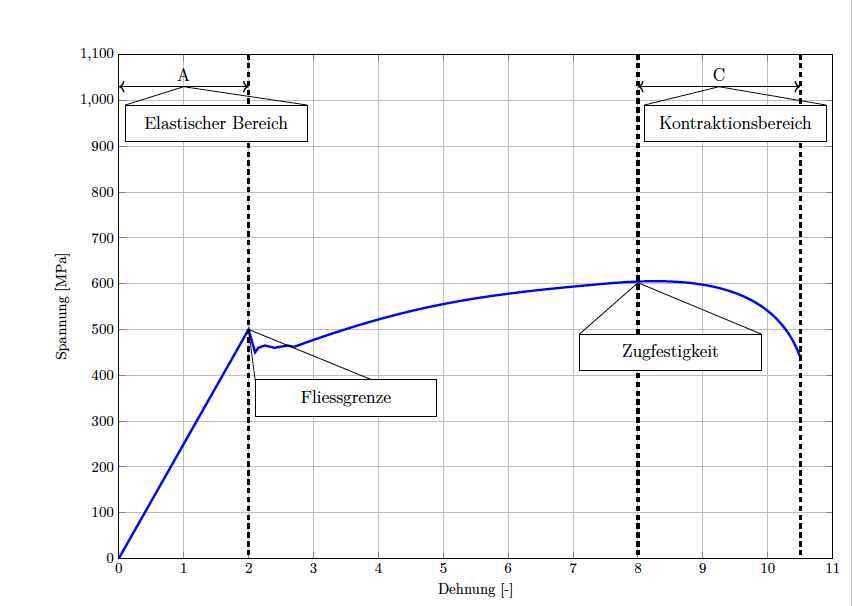
\includegraphics[width=0.8\textwidth]{Lsg}
            \caption{Spannungsdehnungsdiagramm}
            \label{fig:Spannungsdehnungsdiagramm}
        \end{figure}
    \end{solution}

    \question
    Berechnen Sie nun die Fliessgrenze und die Zugfestigkeit der beiden geprüften Stähle.

    \begin{solution}
        Es müssen jeweils diese beiden Formeln verwendet werden:
        \begin{equation*}
            f_{y}  =
            \dfrac{\text{Fliesskraft}}{\text{A}} \approx \FinRes{\myNmm{500}}
        \end{equation*}


        \begin{equation*}
            f_{y}  =
            \dfrac{\text{Höchstlast}}{\text{A}} \approx \FinRes{\myNmm{540}}
        \end{equation*}

    \end{solution}



    \question
    Messen Sie mit einer Schublehre den Durchmesser an der dünnsten Stelle und berechnen Sie die wahre Spannung am Bruchquerschnitt.

    \begin{solution}
        Es werden diese beiden Formeln gebraucht:
        \begin{equation*}
            A = \dfrac{D^2}{4\cdot \pi}
        \end{equation*}

        \begin{equation*}
            \sigma = \dfrac{F_{Hoechstlast}}{A}
        \end{equation*}

    \end{solution}

    %\question
    %Fügen Sie diesen Punkt bei der Skizze aus Aufgabe 7 hinzu.

    \question
    Prüfen Sie, ob die beiden geprüften Stähle die Anfoderungen aus Aufgabe 1 erfüllen.

    \begin{solution}
        Es müssen die Bedingungen über die Fliessgrenze, Zugfestigkeit und Dehnung bei Höchstlast mit den Anforderungen von Tabelle~\ref{tab:stahleigenschaften} erfüllt werden.

    \end{solution}






\end{questions}
\end{document}